%%%%%%%%%%%%%%%%%%%%%%%%%%%%%%%%%%%%%%%%%%%%%%%%%%%%%%%%%%%%%%%%%%%%%
%%                                                                 %%
%% Please do not use \input{...} to include other tex files.       %%
%% Submit your LaTeX manuscript as one .tex document.              %%
%%                                                                 %%
%% All additional figures and files should be attached             %%
%% separately and not embedded in the \TeX\ document itself.       %%
%%                                                                 %%
%%%%%%%%%%%%%%%%%%%%%%%%%%%%%%%%%%%%%%%%%%%%%%%%%%%%%%%%%%%%%%%%%%%%%

%%\documentclass[referee,sn-basic]{sn-jnl}% referee option is meant for double line spacing

%%=======================================================%%
%% to print line numbers in the margin use lineno option %%
%%=======================================================%%

%%\documentclass[lineno,sn-basic]{sn-jnl}% Basic Springer Nature Reference Style/Chemistry Reference Style

%%======================================================%%
%% to compile with pdflatex/xelatex use pdflatex option %%
%%======================================================%%

%%\documentclass[pdflatex,sn-basic]{sn-jnl}% Basic Springer Nature Reference Style/Chemistry Reference Style

\documentclass[sn-basic]{sn-jnl}% Basic Springer Nature Reference Style/Chemistry Reference Style
%%\documentclass[pdflatex,sn-mathphys]{sn-jnl}% Math and Physical Sciences Reference Style
%%\documentclass[sn-aps]{sn-jnl}% American Physical Society (APS) Reference Style
%%\documentclass[sn-vancouver]{sn-jnl}% Vancouver Reference Style
%%\documentclass[sn-apa]{sn-jnl}% APA Reference Style
%%\documentclass[sn-chicago]{sn-jnl}% Chicago-based Humanities Reference Style
%%\documentclass[sn-standardnature]{sn-jnl}% Standard Nature Portfolio Reference Style
%%\documentclass[default]{sn-jnl}% Default
%%\documentclass[default,iicol]{sn-jnl}% Default with double column layout
%%
%%%% Standard Packages
%%<additional latex packages if required can be included here>
\usepackage[authoryear]{natbib}
%    \bibliographystyle{plainnat}
%    \newcommand\citet[1]{%
%        \citeauthor{#1}~[\citenum{#1}]}
%    \newcommand\citep[1]{%
%        [\citenum{#1}]}
%    \newcommand\citeyear[1]{%
%        \citeyear{#1}}
%    \newcommand\citeauthor[1]{%
%        \citeauthor{#1}}
%%    \bibliographystyle{plainnat}
\usepackage{amsmath, amsthm, amssymb, amsfonts}
%%%%

%%%%%=============================================================================%%%%
%%%%  Remarks: This template is provided to aid authors with the preparation
%%%%  of original research articles intended for submission to journals published 
%%%%  by Springer Nature. The guidance has been prepared in partnership with 
%%%%  production teams to conform to Springer Nature technical requirements. 
%%%%  Editorial and presentation requirements differ among journal portfolios and 
%%%%  research disciplines. You may find sections in this template are irrelevant 
%%%%  to your work and are empowered to omit any such section if allowed by the 
%%%%  journal you intend to submit to. The submission guidelines and policies 
%%%%  of the journal take precedence. A detailed User Manual is available in the 
%%%%  template package for technical guidance.
%%%%%=============================================================================%%%%

\jyear{2022}%

%% as per the requirement new theorem styles can be included as shown below
\theoremstyle{thmstyleone}%
\newtheorem{theorem}{Theorem}%  meant for continuous numbers
%%\newtheorem{theorem}{Theorem}[section]% meant for sectionwise numbers
%% optional argument [theorem] produces theorem numbering sequence instead of independent numbers for Proposition
%%\newtheorem{proposition}[theorem]{Proposition}% 
%%\newtheorem{proposition}{Proposition}% to get separate numbers for theorem and proposition etc.
\newtheorem{proposition}[theorem]{Proposition}
\newtheorem{lemma}[theorem]{Lemma}
\newtheorem{corollary}[theorem]{Corollary}
%%
\theoremstyle{thmstyletwo}%
\newtheorem{example}{Example}%
\newtheorem{remark}{Remark}%

\theoremstyle{thmstylethree}%
\newtheorem{definition}{Definition}%

\raggedbottom
%%\unnumbered% uncomment this for unnumbered level heads

\begin{document}

\title[Understanding Environmental Risk Premium of Financing Securities]{Understanding Environmental Risk Premium of Financing Securities: Sovereign Green Sukuk}

%%=============================================================%%
%% Prefix	-> \pfx{Dr}
%% GivenName	-> \fnm{Joergen W.}
%% Particle	-> \spfx{van der} -> surname prefix
%% FamilyName	-> \sur{Ploeg}
%% Suffix	-> \sfx{IV}
%% NatureName	-> \tanm{Poet Laureate} -> Title after name
%% Degrees	-> \dgr{MSc, PhD}
%% \author*[1,2]{\pfx{Dr} \fnm{Joergen W.} \spfx{van der} \sur{Ploeg} \sfx{IV} \tanm{Poet Laureate} 
%%                 \dgr{MSc, PhD}}\email{iauthor@gmail.com}
%%=============================================================%%

\author*[1,3]{\fnm{Aryo} \sur{Sasongko}}\email{aryo@bi.go.id}

\author[2,3]{\fnm{Ali} \sur{Sakti}}\email{a\textunderscore sakti@bi.go.id}

%%\equalcont{These authors contributed equally to this work.}

%%\author[1,2]{\fnm{Third} \sur{Author}}\email{iiiauthor@gmail.com}
%%\equalcont{These authors contributed equally to this work.}

\affil*[1]{\orgdiv{Bank Indonesia Institute}}

\affil[2]{\orgdiv{Islamic Economic and Finance Department}}

\affil[3]{\orgname{Bank Indonesia}, \orgaddress{\street{M.H. Thamrin \#2}, \city{Jakarta}, \postcode{10350}, \state{DKI Jakarta}, \country{Indonesia}}}

%%\affil[3]{\orgdiv{Department}, \orgname{Organization}, \orgaddress{\street{Street}, \city{City}, \postcode{610101}, \state{State}, \country{Country}}}

%%==================================%%
%% sample for unstructured abstract %%
%%==================================%%

\abstract{Green Sukuk and other green financings aim to reduce waste generation and accumulation by reducing environmentally hazardous projects. Sovereign green Sukuk’s issuance has been growing to provide financial returns alongside positive environmental impacts. However, its environmentally-friendly feature price is so unclear that investors can not distinguish between Green and Non-Green Sukuk prices. This research exercises a fundamental asset pricing methodology that analyzes environmental risk. We noticed that unique environmental risks impose Sukuk holders, i.e., systemic and reputation risks. Finally, we simulated these models to cause the risks and price difference.}

%%================================%%
%% Sample for structured abstract %%
%%================================%%

% \abstract{\textbf{Purpose:} The abstract serves both as a general introduction to the topic and as a brief, non-technical summary of the main results and their implications. The abstract must not include subheadings (unless expressly permitted in the journal's Instructions to Authors), equations or citations. As a guide the abstract should not exceed 200 words. Most journals do not set a hard limit however authors are advised to check the author instructions for the journal they are submitting to.
% 
% \textbf{Methods:} The abstract serves both as a general introduction to the topic and as a brief, non-technical summary of the main results and their implications. The abstract must not include subheadings (unless expressly permitted in the journal's Instructions to Authors), equations or citations. As a guide the abstract should not exceed 200 words. Most journals do not set a hard limit however authors are advised to check the author instructions for the journal they are submitting to.
% 
% \textbf{Results:} The abstract serves both as a general introduction to the topic and as a brief, non-technical summary of the main results and their implications. The abstract must not include subheadings (unless expressly permitted in the journal's Instructions to Authors), equations or citations. As a guide the abstract should not exceed 200 words. Most journals do not set a hard limit however authors are advised to check the author instructions for the journal they are submitting to.
% 
% \textbf{Conclusion:} The abstract serves both as a general introduction to the topic and as a brief, non-technical summary of the main results and their implications. The abstract must not include subheadings (unless expressly permitted in the journal's Instructions to Authors), equations or citations. As a guide the abstract should not exceed 200 words. Most journals do not set a hard limit however authors are advised to check the author instructions for the journal they are submitting to.}

\keywords{Islamic finance, Risk management, Climate finance, Environmental-systemic risk premium, Environmental reputation risk premium}

\pacs[JEL Classification]{F64, G12, L14, Q51, Q54}

%%\pacs[MSC Classification]{35A01, 65L10, 65L12, 65L20, 65L70}

\maketitle

%% main text
\section{Introduction}
\label{Introduction}
\subsection{Background}
In this study, we introduce risk-based models for understanding the pricing of Sovereign Green Sukuk, which is a new asset class. This study extends from Sharia-compliant instruments to the risks of environments, operations, and reputations and forms the term structure of interest rates containing these risks. Since June 2018, a green debt class has followed the Green Bond Principles (GBP) stated by the International Capital Market Association (ICMA), which guides transparency to track environmental projects and estimate their impacts. The issuance of sovereign green debt is a part of public policies which encourage domestic firms and the capital market to utilize green-project collateralized assets \citep{monasterolo2018eirin}.

Sukuk characteristics should comply with \emph{Maqasid al-Shariah}, preserving the mother nature, flora and fauna, and place of human beings' lives (\emph{nafs}) \citep{khouildi2018innovative}. Since \citeyear{wilson1997islamic}, \citeauthor{wilson1997islamic} said that the moral criteria of conventional green or ethical investors were similar to that of Islamic, but they had a different underlying moral value system. Furthermore, \citet{charfeddine2016socially} stated that Islamic funds and Socially Responsible Investing (SRI) grew together to be ethical investments, and Islamic funds were the subset of SRI.

Not only should Green Sukuk issuance comply with GBP but also sharia compliance with certain maturity or finite-life but share-like security. The Accounting and Auditing Organization for Islamic Financial Institutions (AAOIFI) defines a Sukuk in Sharia Standard No. 17 as proof of ownership, an undivided share with ownership of specific project assets \citep{hanefah2013sukuk}. Like conventional bonds, some classes of Sukuk securities need the discount rates of the yield curve to calculate the net present value (NPV) of cash flows as a standard pricing methodology \citep{razak2019contracts}. \citet{ahroum2017pricing} implement the Gordon Shapiro model, a division of the NPV model, for pricing the Sukuk Musharakah contract. 

%%Sukuk commonly refers to Sharia-compliant Bond 

In line with \citet{zulkhibri2015synthesis} advice, the research on Sukuk should analyze further into the mainstream of economics and finance. Market risk determines the price of both conventional bonds and Sukuk, including a green-induced price gap that must exist for Sukuk. This research suggests adjusting the term structure of Sukuk yield with environmental risk premiums, and the term structure determines Sukuk pricing.

The traditional theory was that the interest rate contains an inflation rate \citep{fisher1896appreciation}. \citet{rahman2017sovereign} found that the inflation rate could explain the movement of sovereign Sukuk yields using data from 2006 to 2013. \citet{shahida2014predicting} and \citet{ng2019does} found that credit rating shift changed Sukuk price, and Sukuk price contained default risk premium. \citet{safari2013debt} found the firm's risk structure to price corporate Sukuk, such as firm's $\beta$, and credit risk. \citet{awaludin2015sukuk} stated that the Sukuk yield curve also contained risk premium and liquidity premium. In \citeyear{durand1942basic}, \citeauthor{durand1942basic} noted that the \emph{basic yield}, using the current term \citep[pp. 17]{fabozzi2007fixed}, contains a market risk premium comprising a credit risk premium, an inflation risk premium, and a liquidity premium. Like conventional bonds, Sukuk’s yield to maturity (YTM) also contains several layers of risk premiums, including market risk premiums \citep{tariq2007risks,al2013sukuk}.

\subsection{Motivation}

Barely could we associate the potential environmental problem with fundamental market risks, i.e., inflation and credit risks. In \citeyear{meadows1992beyond}, \citeauthor{meadows1992beyond} had implicitly introduced environmental-systemic risk. They said that the population was still growing fast, and people consumed natural resources and produced pollutants at exceeding sustainable rates. Therefore, the young generation would face a declining quantity of food, energy, and production. \citet{nordhaus1994managing} modeled and simulated some governmental climate-change policies. Unfortunately, his analysis revealed that even with advanced technology and tight controls, the existing accumulative waste coupled with massive nonaction on waste generation would inevitably cause immense climate change. \citet{daly2013further} was following and said that economic growth had certain costs, such as climate change, greenhouse gases, and submerged land. \citet{pasqualino2019integrated} developed global food and energy system dynamic models when weather shock (climate change) and increasing population. The input parameters of this model were all in macroeconomic and commodity price variables. At last, \citet{ramani2020addressing} called for the action of U.S. financial regulators. She said that climate change was the source of systemic risk because climate change and extreme weather would devastate the environment, communities, and production facilities.

\citet{schwarcz2008systemic} defined systemic risk as to the ruin of the entire financial system since a triggering event, such as an economic shock or institutional failure, leads to a chain of adverse economic consequences—such as a domino effect on the chain of financial institutions and markets. Environmental damage can also be a spur for these risks, which we use the term \emph{environmental-systemic risk}. Like the financial system, the risk attributes to comovements between ecological problems and other adverse events, which cause a subsequent chain of economic turmoil. The banking and currency systemic contagion could impair innocent and well-behaved banks, countries, firms, and people \citep{kaufman2000banking}, so would the environmental-systemic event. 

Some research articles have mentioned that environmental waste or pollution aggravates the natural region. \citet{liu2020soil} researched the arsenic (As) mining process, causing pollution at significant concentrations in southwest China. The contaminated soil would potentially spoil groundwater. The ecological risk becomes a locally environmental-systemic risk since the groundwater flows everywhere, i.e., surface water and community’s drinking water reservoir. \citet{johannsdottir2019systemic} assessed the potential damages to the arctic area after retreating ice sheets and glaciers since climate change. The situation would initiate economic activities, such as oil and mineral excavations. Maintaining the Arctic ecosystem is also crucial since it supplies nutrition, cultural, social, and economic values. The more the melted ice sheet was, the higher were the activities and natural problems. The excavations could negatively impact various species, ecosystems, traditional communities. These would potentially exacerbate the economic effects and be a regionally environmental-systemic risk.

Despite the locally environmental-systemic risk, some academic works of literature contain the biosphere risk of a potential large-scale regional area and multidimensional crises. \citep{tang2013cold} said that the arctic sea-ice loss changed the atmospheric circulation at high northern latitudes, causing cold winter extremes in the northern hemisphere, including the Siberian continent \citep{ogawa2018evaluating}. The second effect of the loss is a late response of polar stratospheric cooling, which changes ozone concentration and ultraviolet radiation reaching the ground surface \citep{screen2013atmospheric}. The third is varying Arctic climate responses to increasing greenhouse gases \citep{screen2013atmospheric}. The last is sea-level rise, which will rise between 20 cm and 90 cm from 1996 to 2100 \citep{yohe1998sea}. Together with its inhabitants, submerging land causes enormous loss of communities, economy, environment, and culture.

\subsection{Research Gap}
Bonds and Sukuk’s prices reflect all available information \citep{malkiel1970efficient}, including the exposure to environmental-systemic risk. Therefore, investors should have priced the environmental risks exposing all debt securities, green and non-green securities. \citet{broadstock2019time} found that the financial market and economic activities systematically caused a correlation pattern between green and conventional bonds. Environmental-systemic risk should impose across all economic activities and financing contracts; however, \citet{hachenberg2018green} found that green Bonds’ yield was lower than that of non-green bonds. The lower the credit rating was, the larger is their pricing differences, e.g., the yield spread of a single A-rated Bond is as much as 3.88 bps. \citet{zerbib2019effect} found that green bonds of various issuers had an average negative yield premium of 2 bps from conventional bonds.

Furthermore, \citet{cerqueti2021esg} had equity funds data with Morningstar Historical Sustainability Scores’ attributes from 2016 to mid-2018. They concluded that high ESG ranked funds were more resilient than low and less weak to fire-sales spillovers. The reputation risk has tackled that high ESG rated funds have thinner premiums than low ones. \citeauthor{pedersen2020responsible} findings in \citeyear{pedersen2020responsible} that ESG-aware investors earned a higher Sharpe ratio\footnote{Sharpe ratio (SR) measures the investment performance \citep{sharpe1964equilibrium}. It is the ratio between the gap of investor portfolio return ($R_a$) from benchmark return ($R_b$) and their covariance, or: \emph{SR} $=\frac{R_a-R_b}{\sqrt{\sigma^2\left(R_a,R_b\right)}}$.} than ESG-unaware. \citet{alessi2021greenium} said that European green companies’ stocks had a negative risk premium called greenium. Using a stress test scenario, \citeauthor{alessi2021greenium} found that the greener and the more transparent company was, the better was the stock’s yield performance. However, an explanation of these differences has not yet been available. There must be another risk premium attributed to green and non-green securities that we have not yet identified.

\subsection{The Concept of Environmental-Reputation Risk Premium}
Despite the existence of environmental-systemic risk, we need to identify the actors' unique behaviors in interacting with their environment- the reputation risk. Conceiving the reputation risk, we visit the operational risk. According to \citet{solvency2007glossary}, operational risk is a potential loss due to either inadequate internal processes, such as failure of Human Resources systems and management, or external cases, such as legal compensation or fines. \cite{radomska2014operational} said that every firm must have established capabilities to implement strategies to attain its objectives and overcome sustainability threats. The threats might take both internal and external perspectives.

Revisiting operational risk from environmental views, firm’s managers have the internal perspective course of the strategic management process either takes care or casts aside the living world conservation or targets a certain ESG score level. The managers' external views may become a problem after incorrect decisions from the lack of understanding, environmental changes, etcetera. \citet{jarrow2008operational} divided operational risk into two types. In this case, the first type is the loss due to the operating system since the system’s designers did not assume any environmental problem, which might cause supply failure or losing the customer. The second type is agency costs incurred by disagreements between company owners and managers to meet ESG requirements and regulation. A wrong decision, which is the source of operational risk, will trigger the organization’s external, reputational risk.

According to \citet{solvency2007glossary}, reputational risk is the potential adverse publicity regarding the company’s business practices, either accurate or not, which will result in a loss of trust in the company’s integrity. \citet{gormley2011growing} wrote about legal responsibilities when company workers got cancer due to exposure to chemicals due to the work location. This case made a significant negative shock for the company. \citet{gatzert2016assessing} stated that reputational risk would become increasingly important, especially investors and regulators demanded transparency in organizational behavior, and social media was growing. They found that operational loss events had incurred more than fair valuation in the equity market, and researchers considered the excess a reputational loss.

Similar to the relationship between operational and reputation risks, there is also an association between environmental-systemic risk and reputation, specifically environmental-reputation risk—the risk of ESG negligent firms and countries.

\subsection{Research Contribution}

The environmental-systemic and environmental-reputation risks impose on all financial securities, including traditional bonds and green Sukuk. Under systemic events, sustainability projects can have lower reputational costs than non-green projects. In the second chapter, this study models the green Sukuk as explored in other conventional bonds and details the risk premiums' role.

We devised waste generation and accumulative waste models to introduce environmental-systemic risk models, the primary model. The method of environmental-systemic risk premium estimates the remaining capacity of the earth to accommodate accumulative waste before reaching its maximum capacity. We also built a model to estimate the time for the systemic events. Furthermore, we found that people's attention to systemic events depends solely on waste generation.

Given the environmental-systemic event, we established the potential environmental-reputational model. Reputation issues are getting lower with the level of environmental concern. Increasing waste accumulation concurrently accelerates environmental-systemic risk and environmental-reputational risk. The longer the Sukuk maturity, is the higher is the risk premium. We demonstrate the risk premiums, contributing layers within Sukuk’s composite risk premium. Finally, the third chapter concludes the discussion and gives recommendations to develop the green Sukuk market.

\section{Model Development}
\subsection{Waste Generation}
\begin{remark}
Basel Convention on the Control of Transboundary Movements of Hazardous Wastes and Their Disposal \citep{law1989basel} in article two clause one defined a general term of waste as \emph{substances or objects disposed of or intended to be disposed of or were required to be disposed of by the provisions of national law}. Most residue from industrial processes is a hazardous material called pollution. According to the Encyclopedia of Britannica, pollution is the release or removal of materials or substances into nature.
\end{remark}

Previous research showed that there were so many sources of waste. \citet{bruvoll1997future} found that Sweden's manufacturing waste mainly came from material input. However, according to \citet{bandara2007relation}, waste generation was equivalent to population growth and average income. \citet{benitez2008mathematical} determined four crucial factors of residential solid waste, i.e., education level, number of residents, and income. \citet{brock2010green} developed a green Solow model that income and population were pollution sources. \citet{chhay2018municipal} found that the growth of municipal solid waste in China positively related to urban population growth, GDP, and energy consumption. \citet{pasqualino2019integrated} utilized dynamic models to simulate climate-change shocks. Their observation scopes were global food and energy productions and prices. \citet{araiza2020forecast} made the municipal waste forecasting model in Mexico. They found that the most crucial waste generation source was population, followed by income and education level. Therefore, We develop a waste generation model covering all possible sources, i.e., the waste of final products and manufacturing processes.

We consider the population and its economic activities the source of waste, so waste production results from world population and production activities. In \citeyear{copeland1994north}, \citeauthor{copeland1994north} implicitly assumed that the pollution distribution was not moving far away from a pollutant-generating community. In \citeyear{brock2010green}, \citeauthor{brock2010green} developed the Green Solow model, which implicitly represented world pollution. We assumed that pollution production could widely spread to other communities without borders. Like those models of green Solow \citep{brock2010green}, and the final consumption expenditure of households \citep{mazzanti2008waste}, we develop a composite unit of wastes and pollution, which are harmful to nature.

\begin{definition}
	We defined \emph{waste generation} as the aggregate flows of waste and pollution, which are by-products of humans' economic activities. The production of waste and pollution, directly and indirectly, aggravates the environment, social life, and corporate governance (ESG).

	We categorize the components of waste and pollution sources as follows:
	\begin{enumerate}
		\item the aggregate of basic wastes that the garbages of basic needs, $C_B$,
			\begin{equation}\label{cb_detail}
				C_B=\sum_{g=1}^G\,\theta_{B,g} P_g
			\end{equation}
			where $\theta_{B,g}$ is the waste portion of the primary products and conversion of natural destruction unit, $P$ is the population, $g$ the group subindex of basic waste, and $P=\sum_{g=1}^G\, P_g$. 
			\begin{equation}\label{cb}
				C_B=\theta_B P
			\end{equation}
			where $\theta_B$ is the weighted average of waste portion, $\theta_{B,g}$.
			
			Some examples of basic needs waste are plastic waste, electronic waste, cigarette waste, building debris, and organic waste. 
		\item the aggregate amount of non-basic goods or services, $C_L$,
			\begin{equation}\label{cl_detail}
				C_L=\sum_{g=1}^G\,\theta_{L,g} Y_g
			\end{equation}
			where $\theta_{L,g}$ is the waste portion of the non-basic products or services and conversion of natural destruction unit, $Y$ is the income, $g$ the group subindex of non-basic waste, and $Y=\sum_{g=1}^G\, Y_g$.
			\begin{equation}\label{cl}
				C_L=\theta_L Y
			\end{equation}
			where $\theta_L$ is the weighted average of waste portion, $\theta_{L,g}$.
			
			Some examples of non-basic needs waste are lithium-ion battery waste and aircraft exhaust gasses. 
		\item the aggregate of production waste and pollution that the higher the production level is, the higher is the waste, $Y_P$,
			\begin{equation}\label{yp_detail}
				Y_P=\sum_{g=1}^G\,\theta_{P,g} Y_g
			\end{equation}
			where $\theta_{P,g}$ is the waste portion of manufacturing or servicing processes and conversion of natural destruction unit, $g$ the group subindex of manufacturing or servicing processes, and $Y=\sum_{g=1}^G\, Y_g$.
			\begin{equation}\label{yp}
				Y_P=\theta_P Y
			\end{equation}
			where $\theta_P$ is the weighted average of $\theta_{P,g}$.
			
			Examples of waste manufacturing and servicing are coal combustion, mercury contamination, and epoxy-based-ink waste. 
	\end{enumerate}
	The waste sources in Equations \ref{cb_detail}, \ref{cl_detail}, and \ref{yp_detail} can have various categories, such as region, market segmentation, etcetera.
	However, scarcely do we have any detailed data on each group. Instead, we will develop a model with assumed aggregate data.
\end{definition}

\begin{lemma}
	\label{lemma1}
	Since there is no dominant waste producer globally, and all countries generate waste, we can develop a global waste generation model ($G$) using the constant elasticity of substitution (CES) function and waste acceleration model.
\end{lemma}

Proof of Lemma \ref{lemma1} is available in Appendix \ref{secA1}, Equation \ref{simple_gen_waste} shows the waste generation model.

\subsection{Accumulative Waste}
\begin{definition}
	\emph{Accumulative waste} ($A$) is the waste and pollution balance in the world, potentially causing ESG problems.  As an incoming flow, waste generation ($G$) increases the potential problems amid nature always finds a way to heal itself. The remedies of a damaged environment, as an outgoing flow, consist of natural reversion and green technology ($R$).
	\begin{equation} \label{accumulation}
		dA = G dt - dR
	\end{equation}
	where $dR= \text{max}\left(0,\mu_R A dt + \sigma_R A dz\right)$, and $\mu_R \geq 0$, $\sigma_R \geq 0$.
	
	Using Equation \ref{accumulation} and assuming $A > 0$, we derive the expected and the variance of accumulative waste as follow:
	\begin{align} \label{exp_accumulation}
		dA_t=&G_0e^{\left(W-X-\frac{1}{2}V^2\right)t}\left(1+\int\, Vdz+\frac{1}{2}\int\,V^2+0\right)dt-\mu_R A dt -\sigma_R A dz\notag\\
		E_T^Q\left[\frac{dA_t}{dt}\right]=&G_0e^{\left(W-X-\frac{1}{2}V^2\right)t}\left(1+0\right)-\mu_R A_t \notag\\
		E_T^Q\left[A_t\right]=&\frac{G_0}{W-X-\frac{1}{2}V^2+\mu_R}e^{\left(W-X-\frac{1}{2}V^2\right)t} \mbox{ since we assume $A_0=0$.}
	\end{align}
	\begin{align} \label{var_accumulation}
	&	\sigma_t^2\left[\frac{1}{A_t}\frac{dA_t}{dt}\right]=\sigma_R^2\notag\\
	&	\sigma_t^2\left[A_t\right]=e^{\sigma_R^2t}
	\end{align}
Equation \ref{var_accumulation} shows that the variance of accumulative waste is the remedy variance.

The comparison between $A_{t+1}$ and $A_t$ is as follows:\\
\footnotesize
\begin{align}\label{accumulative_comparison}
    \frac{A_{t+1}}{A_t}&=\frac{W_{t}-X_{t}-\frac{1}{2} V_{t}^2+\mu_{R,t}}{W_{t+1}-X_{t+1}-\frac{1}{2} V_{t+1}^2+\mu_{R,t+1}}e^{\left(W_{t+1}-X_{t+1}-\frac{1}{2} V_{t+1}^2\right)\left(t+1\right)-\left(W_{t}-X_{t}-\frac{1}{2} V_{t}^2\right)t}\notag\\
    &=\frac{a}{b}e^{c-d}
\end{align}
\normalsize
Equation \ref{accumulative_comparison} shows that:
\begin{align}
\mbox{if } c-d>0 &
    \begin{cases}
        \frac{a}{b}<1 \mbox{, then } \frac{A_{t+1}}{A_t}<1 \mbox{, and $A_{t+1}$ is decreasing or improving.}\notag\\
        \frac{a}{b}>1 \mbox{, then } \frac{A_{t+1}}{A_t}>1 \mbox{, and $A_{t+1}$ is increasing or worsening.}\notag\\
    \end{cases}
\end{align}
\begin{align}
\mbox{if } c-d<0 &
    \begin{cases}
        \frac{a}{b}>1 &\mbox{, then } \frac{A_{t+1}}{A_t}<1 \mbox{, and $A_{t+1}$ is improving.}\notag\\
        \frac{a}{b}<1 &\mbox{, then } \frac{A_{t+1}}{A_t}>1 \mbox{, and $A_{t+1}$ is worsening.}
    \end{cases}
\end{align}
When $W$, $X$, and $V$ are constant, $c-d$ can be greater than zero as long as $W$ is larger than $X+\frac{1}{2}V^2$. $W$ and $\mu_R$ require increments, and $X$ and $V$ need reduction to shrink $\frac{a}{b}$ and accumulated waste, $A$.
\end{definition}

\begin{figure}[h!]
	\centering
	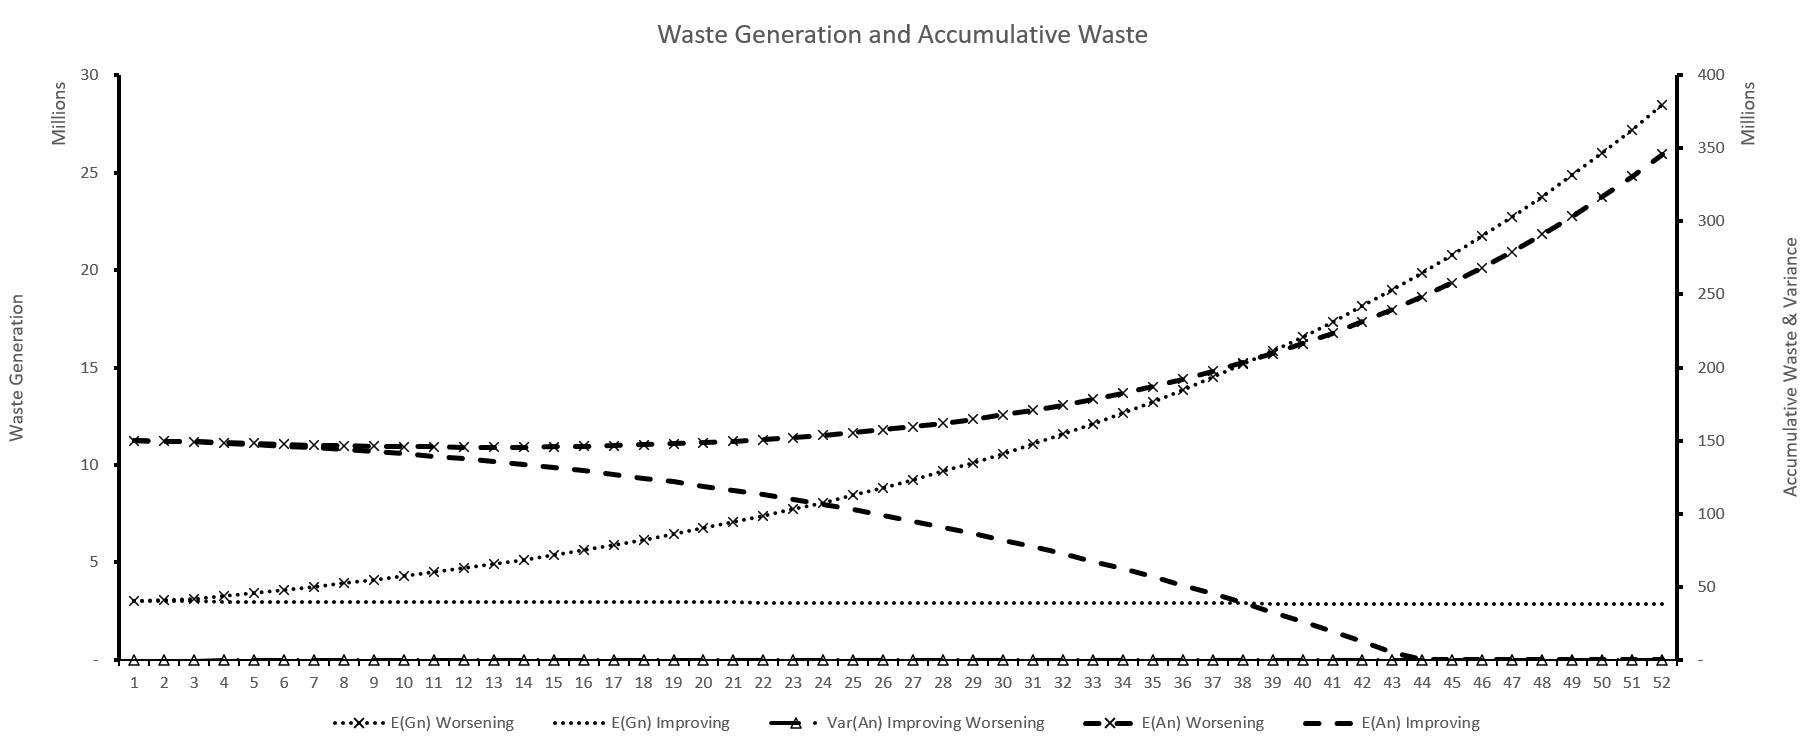
\includegraphics[width=1.0\textwidth]{Fig2_BW}
	\caption{The simulation of expected \emph{waste generation} ($E_t\left(G_n\right)$) and \emph{accumulation} ($E_t\left(A_n\right)$) using Equation \ref{simple_gen_waste}, \ref{exp_accumulation}, and \ref{var_accumulation} from overnight to a hundred years with improving and worsening scenarios. The parameters are $G_0=1000$, $X=0.3$, $V=0.25$, $\mu_R=0.5$, $\sigma_R=0.2$. When the situation worsening with no parameter change, $W>X+\frac{1}{2}V^2$, $W=0.35$ and $W-X-\frac{1}{2}V^2=0.02$. Otherwise, when the situation improving with no parameter change, $W<X+\frac{1}{2}V^2$, $W=0.27$, and $W-X-\frac{1}{2}V^2=-0.06$.}
	\label{fig2}
\end{figure}
Figure \ref{fig2} shows the worsening and improving accumulation simulation in Equation \ref{exp_accumulation}. The deteriorating situation is when the waste generation and accumulation lines are overshooting. The improving line is decreasing or dampening.

\begin{figure}[h!]
	\centering
	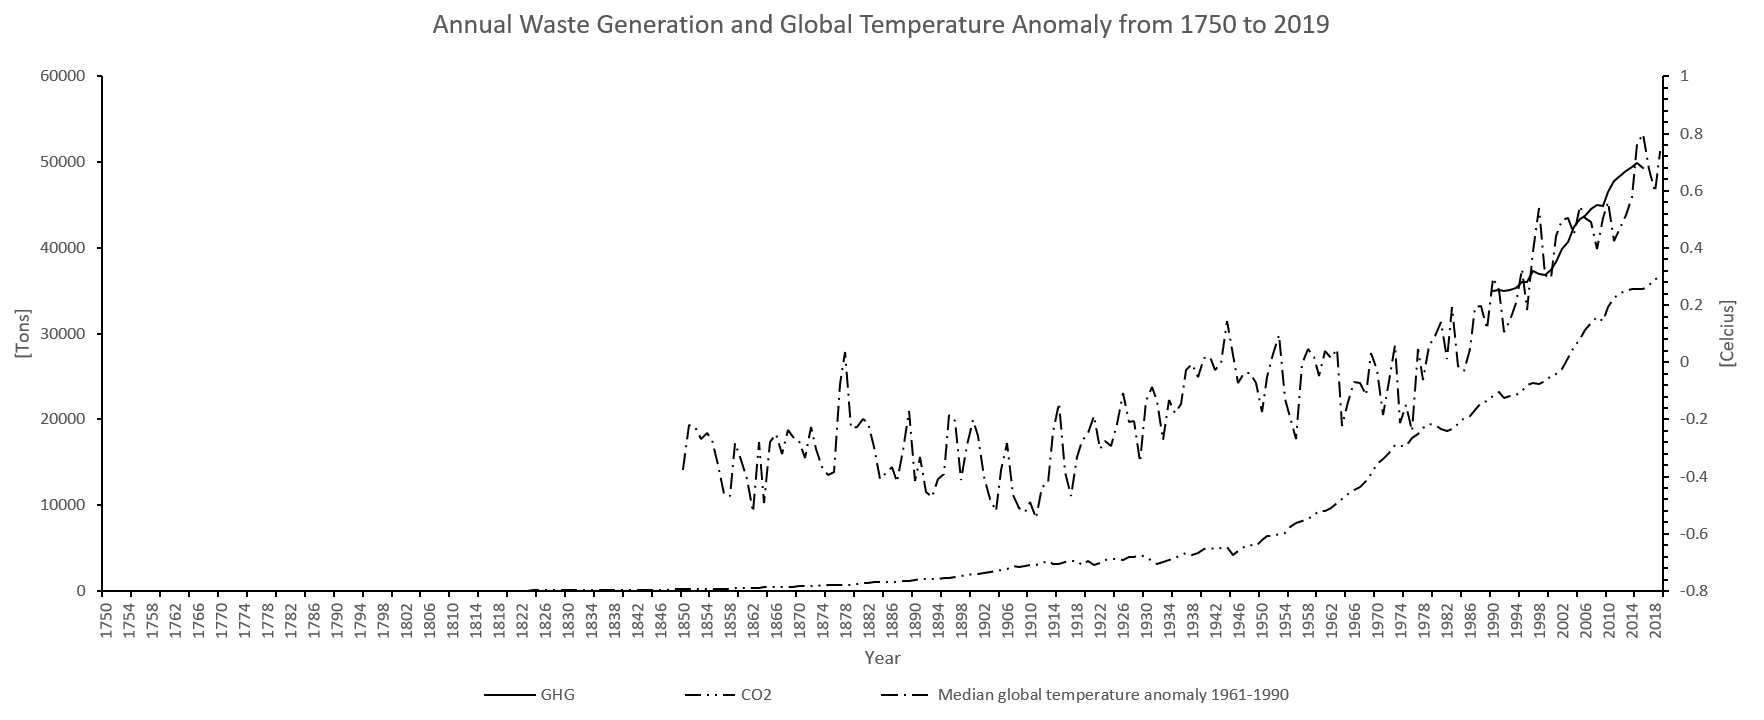
\includegraphics[width=1.0\textwidth]{Waste_Gen_Pic_BW}
	\caption{Waste generation of CO$_2$ and Green House Gasses (GHG) emmisions in tonnes. The temperature gap is in degree Celcius. Source: Our World in Data.}
	\label{fig_waste_gen}
\end{figure}
Unfortunately, Figure \ref{fig_waste_gen} shows that the real world’s accumulative generation is in a positive trend, and we perceive that the state of the earth is deteriorating. There is a common consent to control global $\theta_B$, $\theta_L$, and $\theta_P$ in Equations \ref{cb}, \ref{cl}, and \ref{yp}. Since 11 December 1997, they Kyoto Protocol ratifying countries have managed some actual actions to limit and reduce \emph{waste generation}. They execute standard policies, i.e., carbon tax, carbon emissions trading or European Union Emissions Trading System, Clean Development Mechanism, etcetera. Those variables could have effectively reduced waste and pollution portions in economic activities.
	
\begin{remark}
	Fortunately, an increasing number of asset owners and portfolio managers underline positively impacting society, the environment, and return rates. They have some reasons. \citet{sharfman2008environmental} supported that the green companies could reduce their cost of capital even though their debt capital’s costs were increasing. However, the firms took on higher leverage to get tax subsidies and improve overall economic performances. \citet{pedersen2020responsible} measured investors' preferences using the Sharpe Ratio using Capital Asset Pricing Model (CAPM). There were three-type investors, ESG-aware who prefer to high-ESG score, ESG-unaware, who do not care about ESG score; and ESG-motivated investors, who optimize across three characteristics, i.e., risk and return and ESG score. They found that ESG-aware investors got a higher ratio than ESG-unaware when the ratio was positive.
\end{remark}

\subsection{Environmental-Systemic Risk}
When the world is accumulating waste, the financial markets can gradually monetize and quantify the ESG damages. \citet{nordhaus1977economic} said that an increase in economic activity would have increased the carbon dioxide volume and the earth's temperature. At that time, an increase in the carbon dioxide volume twice could have increased the earth's temperature by 3 degrees Celsius. Some ecologists believe that two degrees of warming could destroy ecosystems on about 13\% of the world's land area, increasing the risk of extinction for many insects, plants, and animals \citep{tollefson2018ipcc}. Moreover, if the community keeps the heating to 1.5 °C, the systemic risk will reduce by half. \citet{leboullenger2017assess} said that climate or environmental-systemic risk was future problems looming over the environment, extended to social, and then to the financial market. Does neither the sky nor the ocean have a physical border. Therefore, pollution flows and spreads out to other parts of the world, triggering environmental-systemic loss.

\begin{definition}
	\emph{Environmental-systemic risk} ($\pi_E$) is the potential event of natural calamity and subsequent ecological disaster when the earth can no longer tolerate any additional waste. The current level of accumulative waste, $A_t$, triggers the systemic risk when $A_t\geq A_S$\footnote{The model based on the length between $A_t$ and $A_s$ is similar to the distance-to-default model \citep{merton1974pricing}.}. However, the systemic event may gradually occur globally, and scientists may debate the $A_S$ level. Still, they can only estimate it, which $A_S\sim N\left(\mu_S,\sigma_S^2\right)$, where $\mu_S$ and $\sigma_S$ are constant.
\end{definition}

\begin{corollary} \label{corollary_2}
	Given the known parameters of Equation \ref{exp_accumulation}, we can estimate the expected time to environmental-systemic events, $\tau$.
\end{corollary}

\begin{proof}{Corollary \ref{corollary_2}}
    We use mechanical distance and speed relationship to bridge between the distance-to-systemic event of the accumulative waste in Equation \ref{exp_accumulation} as distance and the waste generation in Equation \ref{simple_gen_waste} as speed. With constant $W_t$, $X_t$, $V_t$, the expected distance is $E_t\left(D\right)$, is as follows:
    \begin{equation}
        E_t\left(D_\tau\right)=A_s-A_t-\int_t^{\tau} G_k dk
    \end{equation}
    where: \footnotesize
    \begin{align*}
    \int_t^{\tau} G_k dk & =\frac{G_0}{\left(W_t-X_t-\frac{1}{2}V_t^2\right) \left(W_t-X_t-\frac{1}{2}V_t^2+\mu R\right)} \left(e^{\left(W_t-X_t-\frac{1}{2}V_t^2\right)\tau}-e^{\left(W_t-X_t-\frac{1}{2}V_t^2\right)t}\right) \\
    & = A_\tau-A_t
    \end{align*}
    \begin{align}
        \because \: E_t\left(D_\tau\right)&=0 \mbox{ at the event,}\notag\\
        A_s&=A_\tau\notag\\
        \therefore \: E_t\left(\tau\right)&=\frac{1}{W_t-X_t-\frac{1}{2}V_t^2} \ln{\frac{\left(W_t-X_t-\frac{1}{2}V_t^2\right) \left(W_t-X_t-\frac{1}{2}V_t^2+\mu R\right)}{A_s\, G_0}}
    \end{align} \normalsize
\end{proof}

\begin{proposition}\label{proposition_1}
	We can estimate the environmental-systemic risk premium as an additional layer in the term structure of Sukuk yield. The parameters are the probability of the event, $p_{E,n}$, Sukuk’s payoff, which is at recovery level, R, much less than 100\% under the circumstances; otherwise, Sukuk makes a full payment.
\end{proposition}

\begin{proof}{Proposition \ref{proposition_1}}
	In this risk premium model, we have two distributions, i.e., the distribution of current accumulative waste, $A_t$, and the distribution of systemic-accumulative waste, $A_s$, where $A_t\sim N\left(\mu_{A_t},\sigma_{A_t}^2\right)$ in Equations \ref{exp_accumulation} and \ref{var_accumulation}, and $A_s\sim N\left(\mu_{A_s},\sigma_{A_s}^2\right)$.
	
	When accumulative waste worsens,  the longer the time, the higher the probability of the $A_s$ distribution overlapping $A_t$ distribution. Furthermore, the higher is the environmental-systemic likelihood at a certain time $t$, $p_{t}$, or vice versa when it is improving. To find $p_{t}\left(A_s\leq A_t\right)$, we use the subtraction of two distributions as follow:
	\begin{align}\label{prob_systemic}
		p_{t}\left(A_s\leq A_t\right)&=p_{t}\left(A_s-A_t\leq 0\right) \notag\\
		&=p_{t}\left(\left[A_s-A_t\right]-\left[A_s-A_t\right]\leq A_t-A_s\right) \notag\\
		\because \,& z=\frac{\left(\mu_{A_s}-\mu_{A_t}\right)-\left(\mu_{A_s}-\mu_{A_t}\right)}{\sqrt{\sigma_{A_s,A_t}^2}} \notag\\
		& z \sim  N\left(0,1\right) \notag \\
		\therefore \, & p_{t}\left(z\leq A_t-A_s\right)= \,
		\begin{cases}
			1-p_{t}\left(z\leq \frac{\mu_{A_s}-\mu_{A_t}}{\sqrt{\sigma_{A_s,A_t}^2}}\right) \text{ , if } \mu_{A_s}>\mu_{A_t} \\
			p_{t}\left(z\leq \frac{\mu_{A_t}-\mu_{A_s}}{\sqrt{\sigma_{A_s,A_t}^2}}\right) \text{ , if } \mu_{A_s}<\mu_{A_t} \\
		\end{cases}
	\end{align}
	where we assume there is no correlation between $A_t$ and $A_s$, $\rho_{t,s}$.

	We define $p_{n}$ as the probability of an environmental-systemic event at time $n$ given previous time, $n-1$, there is no environmental-systemic loss. 

	All agents face two probable events, either environmental-systemic possibility from time $0$ to time $n$ with conditional probability $P_{n}$ and $R$ payoff or no event with 100\% payoff (Figure \ref{fig3a}). Given two mutually exclusive outcomes of a scenario, where each outcome will happen with a given probability, both probabilities summing to one. Using \citeauthor{von2007theory} utility theorem and lattice model of Figure \ref{fig3a}, we establish an annuity solution of $n$-year Bills containing environmental-systemic risk premium, $\pi_{E,n}$, and another risk premium, $\pi_{O,n}$, as follow:
	\begin{align}\label{env_systemic}
		\frac{1}{\left(1+\pi_{O,n}+\pi_{E,n}\right)^n }=& \frac{100\%\,\Pi_{k=0}^n\,\left(1-p_{k}\right)+R\, \Pi_{k=0}^{n-1},\left(1-p_{k}\right)p_{n}}{\left(1+\pi_{O,n}\right)^n}\notag\\
		\pi_{E,n}=&\left(1+\pi_{O,n}\right) \left(\frac{1}{\sqrt[n]{\Pi_{k=0}^n\,\left(1-p_{k}\right)+R\, \Pi_{k=0}^{n-1},\left(1-p_{k}\right)p_{n}}}-1\right)
	\end{align}
	\begin{figure}[h!]
	\centering
	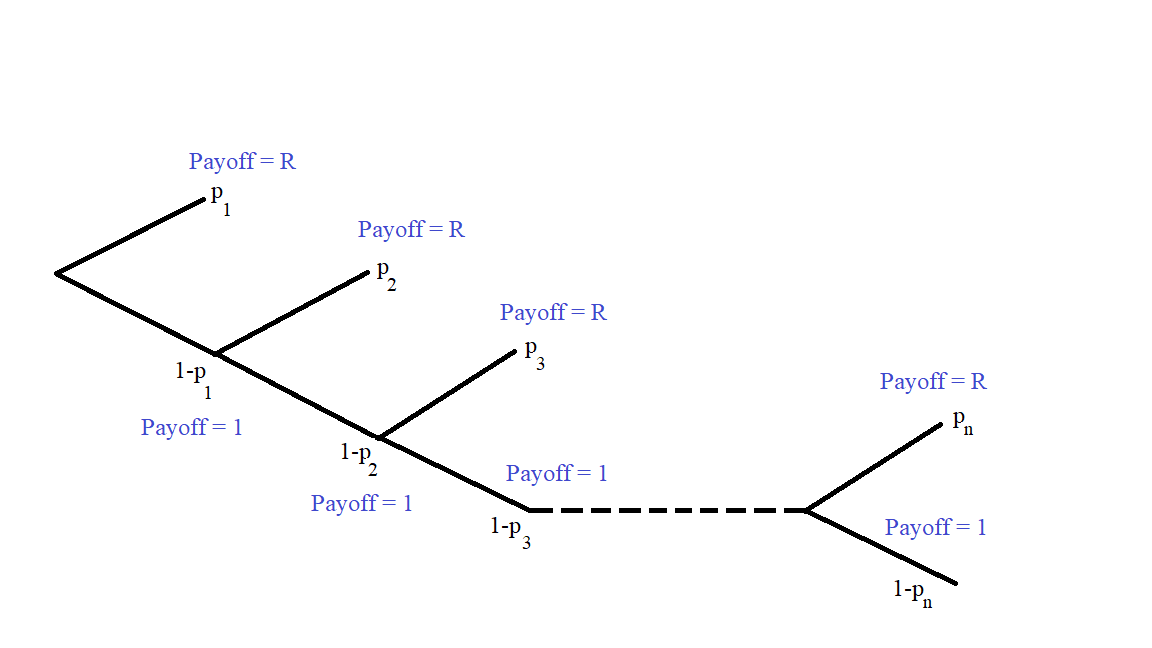
\includegraphics[width=1.0\textwidth]{Fig3a}
	\caption{The probability trees of the environmental-systemic event. $p_n$ is the probability of a systemic event at node-$n$.}
	\label{fig3a}
	\end{figure}
	Figure \ref{fig3a} shows a tree with branches, where each branch represents a period. The event-conditional probability at $n$-th branch is $1-P_{n}$ with $R$ payoff. After the event, the branch is discontinued. Other branches of no event conditional probability, $P_{n}$, are continued in the following years.
	
	\begin{figure}[h!]
		\centering
		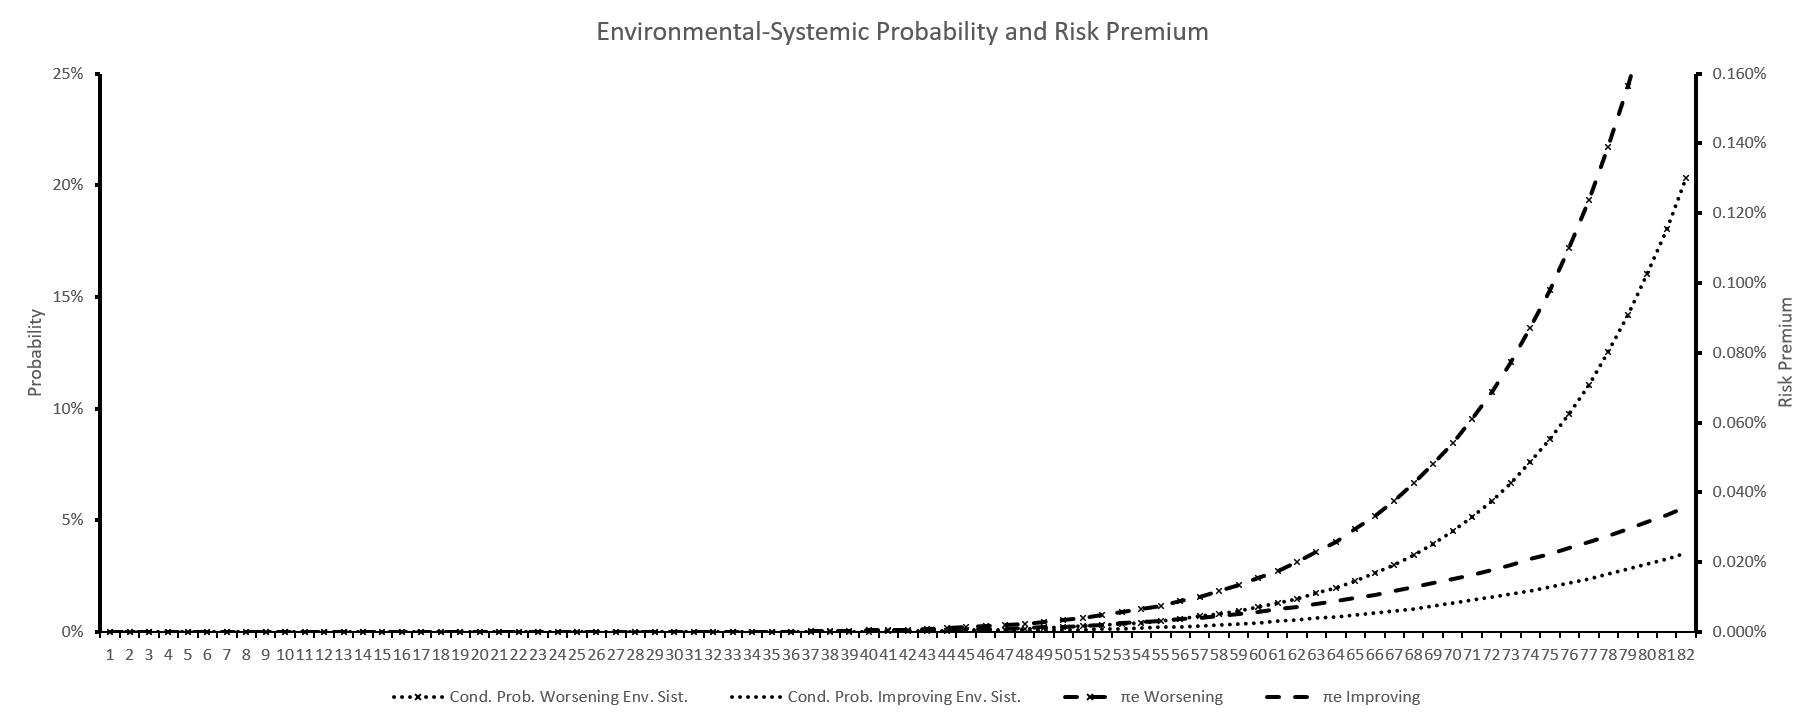
\includegraphics[width=1.0\textwidth]{Fig4_BW}
		\caption{The simulation of environmental-systemic probabilities and risk premiums. The parameters are those of Figure \ref{fig2}, Equation \ref{env_systemic}, $R$=40\%, and the distribution of environmental-systemic event $A_S\sim N\left(15000,1000^2\right)$ from overnight to a hundred years with improving and worsening scenarios.}
		\label{fig3b}
	\end{figure}
	Figure \ref{fig3b} shows the environmental-systemic probability and risk premium with assuming no change of parameters over the years. Since $p_{n}$ is consistently decreasing, the worsening and improving environmental-systemic conditional probabilities, $P_n=\Pi_{k=0}^{n-1},\left(1-p_{k}\right)p_{n}$ of Equation \ref{env_systemic}, drop in the long term.
\end{proof}

\begin{corollary}
	\label{corollary1}
	Economic proliferation drives the expansion of waste generation’s mean and variance. The production can be so fast that nature can no longer recycle or neutralize them, which may worry people. 
\end{corollary}

\begin{proof}{Corollary \ref{corollary1}}
    We will use the absolute risk aversion, $ARA$, model of \citet{pratt1978risk} to reckon people’s apprehensions. The model requires a utility function that gauges personal pleasure or consumer preference, positively affecting communities. The utility of waste has adverse outcomes to the earth instead. The Arrow-Pratt measure of the absolute risk aversion of this utility function is as follows: 
    \begin{equation}\label{ARA}
        ARA_t=-\frac{u^{"}\left(A_t, A_s\right)}{u^{'}\left(A_t, A_s\right)}
    \end{equation}
    where $u\left(A_t, A_s\right)$=$\left(1-p\right) \frac{A_t^{1-\eta}}{1-\eta}$+$p \frac{A_s^{1-\eta}}{1-\eta}$ is a combination of \citeauthor{von2007theory} and isoelastic utility functions in both systemic events with probability $p$ and non-event with probability $1-p$ (Figure \ref{fig3a}), and $\eta$ is the degree of risk aversion.
    
    The derivation of ARA measure becomes as follows:
    \begin{equation}\label{ARA2}
        ARA_t=-\frac{\eta}{A_t}
    \end{equation}

    \begin{align}\label{ARA3}
    \because \: & \mbox{People relief when } ARA_{t+1}\geq ARA_t \mbox{, otherwise people discomfort} \notag\\
    \therefore \: &\mbox{People concern when } \frac{ARA_{t+1}}{ARA_t}\leq 1 \notag\\
        &\mbox{People feel at ease when } \frac{ARA_{t+1}}{ARA_t} > 1 
    \end{align}

    \begin{align}\label{ARA4}
        \because \: &\frac{ARA_{t+1}}{ARA_t}=\frac{W_t-X_t-\frac{1}{2}V_t^2+\mu_R}{W_{t+1}-X_{t+1}-\frac{1}{2}V_{t+1}^2+\mu_R}e^{W_{t+1}-W_t-X_{t+1}+X_t-\frac{1}{2}V_{t+1}^2+-\frac{1}{2}V_t^2} \notag\\
        &\mbox{Assuming } \mu_R \mbox{ is constant,} \notag\\
        \therefore \: & \mbox{People bother when } W_{t+1}-X_{t+1}-\frac{1}{2}V_{t+1}^2 < W_t-X_t-\frac{1}{2}V_t^2 \notag\\
        & \mbox{People relax when } W_{t+1}-X_{t+1}-\frac{1}{2}V_{t+1}^2 \geq W_t-X_t-\frac{1}{2}V_t^2
    \end{align}
\end{proof} 
Equation \ref{ARA4} shows that people’s environmental anxiety solely depends on the growth of waste accumulation which resembles Equation \ref{accumulative_comparison} but regardless of a large number $A_s$. Figure \ref{fig_waste_gen} exhibits that the accumulative wastes of CO$_2$ and GHG in 2018 are increasing, disturbing people.

\subsection{Environmental Reputation Risk}
\begin{remark}
	Most developed countries have their environmental agency. The agency is the source of information to adopt, implement, evaluate some policies, and enforce the law in some countries. In the United States, the Environmental Protection Agency (EPA) is an independent governmental body established in July 1970. It has the power to issue regulations, such as the Clean Air Act, the Clean Water Act, and the Oil Pollution Act. It also has the authority to fine, to give sanctions, to decide other measures. In European countries, the European Economic Community established European Environmental Agency (EEA). Its management board comprises representatives from its 33 member states in the European Economic Community. Its environmental policy must relate to its member’s domestic policies and other international policies. EEA does not have any enforcing law, but it has revealed some ecological problems in the countries, such as implementing Common Agricultural Policy, Common Fisheries Policy, and Water Framework Directive. 
	%%Like the operational-risk-triggered reputational risk, the environmental-systemic risk is the source of environmental-reputational risk. The environmental-systemic loss event initiates problems for companies from isolated areas to large regions. Then, the environmental-reputational risk is following the event. Since ESG risk score measures a company’s attention on and subjection to ESG-related issues, we assume that the reputational loss depends on the ESG rating and score. The more the company complies with obligations for environmental impacts is the lower is the environmental-reputational risk.
\end{remark}

Although nature conservation gets increasing attention from governments, investors, and other organizations, any party is growing concerned about hiding the correct information or capitalizing on this positive trend. \citet{hansen2007scientific} mentioned \emph{scientific reticence} as that scientists had detained the information of greenhouse gas-induced sea level rise, which may level up to a meter by the end of this century. The disadvantage of this constraint is that the government may not prevent the massive floods scientists have previously predicted.

Additionally, vague government regulations drive \emph{greenwashing}. According to \citet{delmas2011drivers}, \emph{greenwashing} is the act of deceiving investors using fake nature conservation (company-level greenwashing) or misinforming customers about the natural benefits of a product or service (product-level greenwashing). Greenwashing brings risks, such as immediately damaging the environment, public distrust in environmentally friendly products and ecologically responsible companies, and harms social welfare. \citet{kim2011strategic} compared reduction reports of the United States' Department of Energy’s Voluntary Greenhouse Gas Registry to the actual emissions of 98 electric power companies. Unfortunately, these companies made selective disclosures of positive environmental outcomes while withholding negative results. \citet{dunn2018assessing} had stated that any company that worked without taking care of the environment, such as high-level emitting of carbon, might get a potential future problem, such as a carbon tax imposed, which is the environmental-reputational risk.

Therefore, ICMA regulated that green bonds' issuers should appoint external review providers to confirm their operational procedures meet with all the core components of the respective Principles, such as GBP. \citet{fatica2021pricing} said that investors could not identify a clear tie between the green bond issued by financial institutions and any specific collateralized green investment project. And, they found that green bonds' issuers that previously had external review assessment benefited from lower debt costs than self-labeled companies.

\begin{remark}
	Adopting ESG direction, some managers may decide not to meet all required categories completely. There are some rating and tool systems to assess the compliance level of a construction project. There are four predominant areas having assessment systems, i.e., the United States, Brazil, Canada, and India, which follow the Leadership in Energy and Environmental Design system (LEED). Moreover, Australia and New Zealand develop the Green Star system. The United Kingdom has the Building Research Establishment Environmental Assessment Method (BREEAM) system. Japan implements the Comprehensive Assessment System for Building Environmental Efficiency (CASBEE). The project’s owner who meets satisfying quality and performance will receive an ESG-compliance certificate with the assessment. Each system has its rating scores, e.g., LEED has six assessment scores, i.e., outstanding, excellent, very good, good, pass, and unclassified. According to \citet{say2008sustainable}, the rating systems create economic, environmental, health and community benefits.
\end{remark}

\begin{definition}
	According to Cambridge Dictionary, \emph{Reputational risk} is a problem that comes from public opinion based on past stories. People profoundly perceive that a company, a country, or a region would have unanticipated legal costs or lost firm value \citep{KUMAR201461}. Like reputation risk, we define environmental reputation risk as either a possible disclosure that an entity's procedures or facilities do not meet its green norms or a pre declaration that an entity would not meet some of the green bars. Financial markets and communities may estimate the risk from its histories. Let $\mathbf{x}$ is a conformance gap vector between green necessity and actual implementation, which each $x_i \in \left(-\infty,\infty\right)$ ranges from less than expected with a negative value, about right or zero gaps, to more than expected with a positive value. The odds of a potential reputational problem given systemic event with logistic regression function is, $\pi_{R,n}\left(y\mid p_{E,n}=1\right)=\frac{1}{1+e^{-y}}$, where $y = \mathbf{x}^T \mathbf{\beta}$, and $\beta\geq 0$ is the weight of each categorical compliant gap.
\end{definition}

\begin{proposition} \label{proposition_2}
	The higher the green-compliance score of financing project, the lower the environmental reputation risk, $\pi_{R}$. Therefore, the green project must suffer less than that of conventional.
\end{proposition}

\begin{proof}{Proposition \ref{proposition_2}}
	Similar to Proposition \ref{proposition_1}, we have two distributions, i.e., the current accumulative-waste distribution (Equations \ref{exp_accumulation}, \ref{var_accumulation}, and $A_n\sim N\left(\mu_{A_n},\sigma_{A_n}^2\right)$) and the estimated environmental-systemic distribution, $A_s\sim N\left(\mu_{A_s},\sigma_{A_s}^2\right)$.
	
	We assume that the higher the green compliance score, the lower the spotting of another critical non-compliance. Moreover, the size of reputational penalties, $F\left(S\right)$, depends on ESG-compliant scoring, $S$, where $F\left(S\right) \leq R$.
	
	There are two possibilities at time $t$ of environmental-systemic risk. It happens with conditional systemic-event probability $p_{E,n}$ with $R$ payoff and imposes $F\left(S\right)$ fines or does not occur with 100\% payoff without any penalty. Using \citeauthor{von2007theory} utility theorem and a lattice model of Figure \ref{fig3a}, we establish $n$-year Bills containing environmental-systemic risk premium, $\pi_{E,n}$, and other risk premiums, $\pi_{O,n}$, and environmental-reputational risk premium, the annual $\pi_{R,n}$ as follows:
	\footnotesize
	\begin{align}\label{reputation}
		\frac{1}{\left(1+\pi_{O,n}+\pi_{E,n}+\pi_{R,n}\right)^n }=& \frac{100\%\,\Pi_{k=0}^n\,\left(1-p_{E,k}\right)+\left(R-F\left(S\right)\right) \,\Pi_{k=0}^{n-1}\,\left(1-p_{E,k}\right)p_{E,n}}{\left(1+\pi_{O,n}+\pi_{E,n}\right)^n}\notag\\
		\pi_{R,n}=\left(1+\pi_{O,n}+\pi_{E,n}\right)& \left(\frac{1}{\sqrt[n]{\Pi_{k=0}^n\,\left(1-p_{E,k}\right)+\left(R-F\left(S\right)\right) \,\Pi_{k=0}^{n-1}\,\left(1-p_{E,k}\right)p_{E,n}}}-1\right)
	\end{align}
	\normalsize
	Equation \ref{reputation} shows that the lower $S$, is the higher is $F$, and is the higher is the environmental-reputational risk premium.
\end{proof}
	
	\begin{figure}[h!]
		\centering
		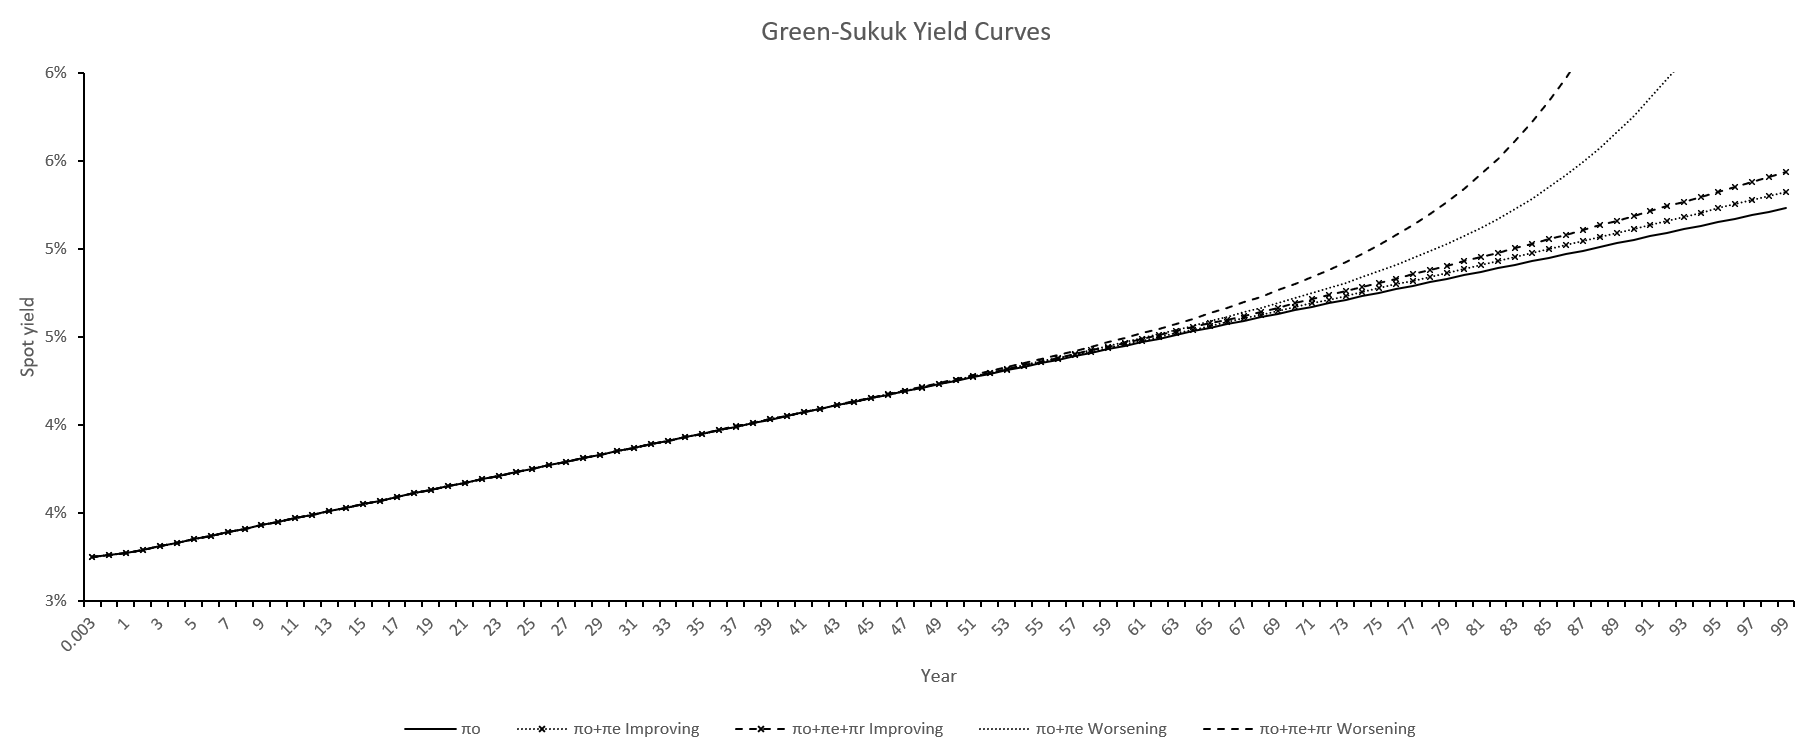
\includegraphics[width=1.0\textwidth]{Fig5_BW}
		\caption{The environmental-systemic and environmental-reputational risk premiums' simulations using Equation \ref{env_systemic} and \ref{reputation} from overnight to a hundred years with improving and worsening scenarios. The parameters are those of Figure \ref{fig2}, $\pi_o$ is a ramp function from 3.25\% to 5.25\% from time 0 to 100 years, and $R-F\left(S\right)$ = 5\%.}
		\label{fig6}
	\end{figure}

Figure \ref{fig6} shows the yield curves. It contains some risk premiums, i.e., environmental-systemic ($\pi_{E}$), environmental-reputational ($\pi_{R}$) with constant parameters. The increasing risks decrease prices since the market expects systemic losses and reputational penalties ($F\left(S\right)$) concurrently: the lower the reputation risk premium ($\pi_{R}$), the more resilient and stable the prices. Under environmental circumstances, the less the entity’s green compliance ($S$), the higher the penalty.

\section{Conclusion and Recommendation}
\subsection{Conclusion}
In this study, we have established the models of environmental systemic and environmental reputational risks and the roles of their premiums in risk-based pricing. These fundamental models address the environment risk premium in all types of financial contracts, either conventional or shariah, and green or brown securities. Including sovereign debts, their essential risk premiums are economic fundamental and environmental.

Our model starts from economic activities that consist of consumption activities and services or manufacturing processes leading to incremental waste generation and rising accumulative waste. Unfortunately, this accumulation is too large that the available green technology and natural remedy can not compensate for these activities. Together with rising temperatures, these increments are a cause of concern for people. At the threshold levels, the earth loses the ability to recover and hold all the accumulative waste.

The common environmental-systemic risk imposes all financial contracts; however, the unique environmental reputation risk has different responsibilities in each issuing country and firm. We assumed that environmental-systemic events would occur together or almost simultaneously in most regions by constructing an environmental-systemic risk model. Such circumstances will mark the beginning of an unwanted change in the biosphere or environmental-systemic loss. In contrast to environmental-systemic risk, the environmental-reputational risk exposes firms to varying degrees depending on the ESG score.

\subsection{Recommendation}
There are three specific methods for decelerating waste generation and lowering accumulative waste. First, scientists need to improve green technology. Better technology refreshes the parameters of waste generation and accumulative pollution. In turn, the new parameters reduce the probability of an environmental-systemic event. The second method is to follow SRI procedures and get positive endorsements and testimonials from external reviewers when issuing securities. Sukuk has inherently been compatible with the procedures to support environmental-reputational mitigation, comply with Maqasid al-Shariah, and contribute to the welfare of society and a cleaner environment. The final method involves pursuing or legally enforcing the issuers of securities to publish their sustainability disclosures and ESG scores. Market participants need this transparency to assess the ESG compliance and environmental reputation of individual entities and the nation.

We expect future research to develop either an aggregate value or an index of accumulative waste with access to all the required waste and pollution data and biochemistry and ecological processes that damage the environment. Researchers can use the index and our theoretical development to use or develop models to determine the time gap of environmental systemic and reputational events. Knowing the increment of accumulative waste, people and communities comprehend the misfortune situation and avert the systemic crisis.

Environmental protector/regulator needs to manage and publicly provide transparent ESG disclosures from external and internal auditors. The clearness will benefit project managers and investors. The managers will have feedback on their environmentally friendly business practices. Furthermore, good corporate governance will attract relevant stakeholders, such as existing and potential customers, investors, suppliers, and regulators. The financial market gets sustainability-compliant information to assess country’s and firm’s reputations. Judging these reputations, investors and other market participants can appraise their green instruments, including green Sukuk and environmental reputation risk premiums.

\backmatter

%%\bmhead{Supplementary information}

%%If your article has accompanying supplementary file/s please state so here. 

%%Authors reporting data from electrophoretic gels and blots should supply the full unprocessed scans for key as part of their Supplementary information. This may be requested by the editorial team/s if it is missing.

%%Please refer to Journal-level guidance for any specific requirements.

\bmhead{Acknowledgments}

This research was impossible without the support of the Bank Indonesia Institute-Bank Indonesia. We are immensely grateful to Mr. Reza Anglingkusumo, the Executive Director of Bank Indonesia, for his comments on an earlier version of the manuscript.

\section*{Declarations}

Some journals require declarations to be submitted in a standardised format. Please check the Instructions for Authors of the journal to which you are submitting to see if you need to complete this section. If yes, your manuscript must contain the following sections under the heading `Declarations':

\begin{itemize}
\item Funding
\item Conflict of interest/Competing interests (check journal-specific guidelines for which heading to use)
\item Ethics approval 
\item Consent to participate
\item Consent for publication
\item Availability of data and materials
\item Code availability 
\item Authors' contributions
\end{itemize}

\noindent
If any of the sections are not relevant to your manuscript, please include the heading and write `Not applicable' for that section. 

%%===================================================%%
%% For presentation purpose, we have included        %%
%% \bigskip command. please ignore this.             %%
%%===================================================%%
\bigskip
\begin{flushleft}%
Editorial Policies for:

\bigskip\noindent
Springer journals and proceedings: \url{https://www.springer.com/gp/editorial-policies}

\bigskip\noindent
Nature Portfolio journals: \url{https://www.nature.com/nature-research/editorial-policies}

\bigskip\noindent
\textit{Scientific Reports}: \url{https://www.nature.com/srep/journal-policies/editorial-policies}

\bigskip\noindent
BMC journals: \url{https://www.biomedcentral.com/getpublished/editorial-policies}
\end{flushleft}

\begin{appendices}

\section{Proof of Lemma \ref{lemma1}}\label{secA1}

	The CES model with those three-category materials is as follows:
	\begin{equation}
		\label{CES}
		G=\sum_{k=1}^K\,\left( \frac{x_{B,k}}{K}C_{B,k}^\rho + \frac{x_{L,k}}{K}C_{L,k}^\rho  + \frac{x_{P,k}}{K}Y_{P,k}^\rho\right)^\frac{1}{\rho}
	\end{equation}
	where $\rho$ is a substitution rate, $k$ is a subindex of a country, $K$ is the number of countries in the world, $x_{B,k} \in \left[0,1\right]$ is the share parameter of basic consumption waste, $x_{L,k} \in \left[0,1\right]$ is the share parameter of non-basic consumption waste, and $x_{P,k} \in \left[0,1\right]$ is the share parameter of by-product waste.
	
	\begin{align}
		\label{CobbDouglas}
		\because \; &\text{waste sources are non substitutible, } \, \rho \approx 0 \notag\\
		\therefore \;  &\text{Equation \ref{CES} becomes: }\, \lim\limits_{\rho \to 0} G = \lim\limits_{\rho \to 0} \, \sum_{k=1}^K\,\left( \frac{x_{B,k}}{K}C_{B,k}^\rho + \frac{x_{L,k}}{K}C_{L,k}^\rho  + \frac{x_{P,k}}{K}Y_{P,k}^\rho\right)^\frac{1}{\rho} \notag\\
		\; & G= \Pi_{k=1}^K\,\left(C_{B,k}^{x_{B,k}} C_{L,k}^{x_{L,k}} Y_{P,k}^{x_{P,k}} \right)
	\end{align}
	
	We can split Equation \ref{CobbDouglas} to measure the waste production of a certain country from the rest of the world. The waste contribution from a country, “1”, is as follow:
	\begin{align}
		\because \:& G= \left(C_{B,1}^{x_{B,1}} C_{L,1}^{x_{L,1}} Y_{P,1}^{x_{P,1}}\right) \,\Pi_{k=2}^K\,\left(C_{B,k}^{x_{B,k}} C_{L,k}^{x_{L,k}} Y_{P,k}^{x_{P,k}} \right) \notag \\
		\therefore \:& G_1 =\frac{G}{\Pi_{k=2}^K\,\left(C_{B,k}^{x_{B,k}} C_{L,k}^{x_{L,k}} Y_{P,k}^{x_{P,k}} \right)}
	\end{align}
	
	We can use log-weighted average method to simplify the model of world waste production as follow:
	\begin{align}
		\because \; & G_1^\frac{x_1}{K}\,G_2^\frac{x_2}{K}\,G_3^\frac{x_3}{K}\,\ldots\,G_K^\frac{x_K}{K}=G_T \text{, such that } 
		\frac{x_1}{K}+\frac{x_2}{K}+\frac{x_3}{K}+\ldots+\frac{x_K}{K}=100\%\notag\\
		\therefore \; & K \ln{G_T} = x_1 \ln{G_1} +x_2 \ln{G_2} +x_3 \ln{G_3} +\ldots+x_K \ln{G_K} \notag\\
		& \ln{G_T}=\frac{\Pi_{k=1}^K\,x_k\ln{G_k}}{K}
	\end{align}
	Including each production factor:
	\begin{align}
		\label{each_prod_factor}
		\because \; & C_1^\frac{x_1}{K}\,C_2^\frac{x_2}{K}\,C_3^\frac{x_3}{K}\,\ldots\,C_K^\frac{x_K}{K}=C_T^{x_T} \text{, such that } 
		\frac{x_1}{K}+\frac{x_2}{K}+\frac{x_3}{K}+\ldots+\frac{x_K}{K}=x_T\notag\\
		\therefore \; & Kx_T \ln{C_T} = x_1 \ln{C_1} +x_2 \ln{C_2} +x_3 \ln{C_3} +\ldots+x_K \ln{C_K} \notag\\	
		& \ln{C_T}=\frac{\Pi_{k=1}^K\,x_k\ln{C_k}}{Kx_T}
	\end{align}
	Therefore, we can express the waste flows all over the world, Equation \ref{CobbDouglas}, as:
	\begin{equation}
		\label{waste_flow}
		G=C_B^{x_{B,T}} C_L^{x_{L,T}} Y_P^{x_{P,T}} 
	\end{equation}
	where according to Equation \ref{each_prod_factor} $C_B=\frac{\Pi_{k=1}^K\,x_{B,k}\ln{C_{B,k}}}{Kx_{B,T}}$, $C_L=\frac{\Pi_{k=1}^K\,x_{L,k}\ln{C_{L,k}}}{Kx_{L,T}}$, and $Y_P=\frac{\Pi_{k=1}^K\,x_{P,k}\ln{C_{P,k}}}{Kx_{P,T}}$.
	
	We develop a waste acceleration model ($dG$) from Equation \ref{waste_flow} to get its component specification. The economic growth (Equations \ref{cb_detail}, \ref{cl_detail}, and \ref{yp_detail}) pushes the waste and pollution of Equation \ref{waste_flow}. The partial stochastic differential equation of waste generation is as follow:
	\begin{align}
		dG=&\frac{\partial G}{\partial C_B}dC_B + \frac{\partial G}{\partial C_L}dC_L + \frac{\partial G}{\partial Y_B}dY_P
		+ \frac{1}{2} \frac{\partial^2 G}{\partial C_B^2}dC_B^2 + \frac{1}{2} \frac{\partial^2 G}{\partial C_L^2}dC_L^2 + \frac{1}{2} \frac{\partial^2 G}{\partial Y_P^2}dY_P^2 \notag\\
		&+ \frac{1}{2} \frac{\partial^2 G}{\partial C_B\partial C_L}dC_BdC_L + \frac{1}{2} \frac{\partial^2 G}{\partial C_B\partial Y_P}dC_BdY_P + \frac{1}{2} \frac{\partial^2 G}{\partial C_L\partial Y_P}dC_LdY_P
	\end{align}

	\begin{align}
			\text{where:}\: & \frac{\partial G}{\partial C_B}=x_B\frac{G}{C_B}       & \text{, and } & \frac{\partial^2 G}{\partial C_B^2}=x_B\left(x_B-1\right)\frac{G}{C_B^2}                         \notag\\
			& \frac{\partial G}{\partial C_L}=x_L\frac{G}{C_L}                     & \text{, and } & \frac{\partial^2 G}{\partial C_L^2}=x_L\left(x_L-1\right)\frac{G}{C_L^2}                         \notag\\
			& \frac{\partial G}{\partial Y_P}=x_P\frac{G}{Y_P}                     & \text{, and } & \frac{\partial^2 G}{\partial Y_P^2}=x_P\left(x_P-1\right)\frac{G}{Y_P^2}                         \notag\\
			& \frac{\partial^2 G}{\partial C_B\partial C_L}=x_Bx_L\frac{G}{C_BC_L} & \text{, and } & \frac{\partial^2 G}{\partial C_B\partial Y_P}=x_Bx_P\frac{G}{C_BY_P}  \notag\\
			& \frac{\partial^2 G}{\partial C_L\partial Y_P}=x_Lx_P\frac{G}{C_LY_P}    \notag                                                
	\end{align}

	Because $G$ depends on a production level, we analytically describe the Cobb-Douglas production or income function ($Y$). $Y$ is a stochastic exponential process as follows:
	\begin{equation}\label{GDP}
		Y=K^\alpha L^{1-\alpha}
	\end{equation}
	where $K$ is an investment or a capital stock variable, $L$ is a labor variable, and $\alpha$ is a shared parameter.
	$P$ (population), $L$, and $K$ are processes following stochastic differential equations (SDEs). They have a finite horizon with $t \in [0,T]$ on filtered probability space $\left(\Omega, \mathbb{F}, \{\mathbb{F}_t\}, \mathbb{P}\right)$ with $\mathbb{P}$ denotes statistical probability measure, and $\mathbb{Q}$ denotes martingale probability measure. These variables are as follows:
	\begin{align}
		dP=& \mu_P P dt + \sigma_P P dt \notag \\
		dL=& \mu_L L dt + \sigma_L L dt \notag \\
		dK=& \left(sY-\delta K\right) dt + \sigma_K K dt \notag
	\end{align}
	where $s$ is a reinvestment rate, and $\delta$ is a depreciation rate, $dz$ is a Brownian motion with normally distributed noise, i.e., $dz\sim N\left(\mu,\sigma^2\right)$, $\mu$ is the drift, and $\sigma$ is the standard deviation, in which both variables are constant.
	
	We also get some stochastic differential equations of $C_B$, $C_L$, and $Y_P$ are stochastic exponential processes from Equations \ref{cb}, \ref{cl}, \ref{yp}, and \ref{GDP}, as follows:
	\begin{align}
		dC_B=& \theta_P \left(\mu_P P dt + \sigma_P P dz_P\right) \notag\\
		dC_B^2=& \theta_P^2 \sigma_P^2 P^2 dt\notag\\
		dC_L=& \theta_L Y \left(\left(\alpha \left(s\frac{Y}{K}-\delta\right)dt + \sigma_K dz_K\right)+\left(1-\alpha\right)\left(\mu_L dt+\sigma_L dz_L\right)\right.\notag\\  &\left. +\frac{1}{2}\alpha\left(\alpha-1\right)\left(\sigma_K^2+\sigma_L^2-\sigma_K\sigma_L\rho_{K,L}\right)dt\right) \notag\\
		dC_L^2=& \theta_L^2 Y^2\left(\alpha^2\sigma_K^2+\left(1-\alpha\right)^2\sigma_L^2+2\alpha\left(1-\alpha\right)\sigma_K\sigma_L\rho_{K,L}\right)dt \notag\\
		dY_P=& \theta_P Y \left(\left(\alpha \left(s\frac{Y}{K}-\delta\right)dt + \sigma_K dz_K\right)+\left(1-\alpha\right)\left(\mu_L dt+\sigma_L dz_L\right)\right.\notag\\ & \left.  +\frac{1}{2}\alpha\left(\alpha-1\right)\left(\sigma_K^2+\sigma_L^2-\sigma_K\sigma_L\rho_{K,L}\right)dt\right) \notag\\
		dY_P^2=& \theta_P^2 Y^2\left(\alpha^2\sigma_K^2+\left(1-\alpha\right)^2\sigma_L^2+2\alpha\left(1-\alpha\right)\sigma_K\sigma_L\rho_{K,L}\right)dt \notag
	\end{align}
	We can get the expected-exponential drift of waste generation, $G$-a stochastic exponential process, as follows:
	\begin{align}\label{wg_mean}
		E_t^Q\left[\frac{1}{G}\frac{dG}{dt}\right]=&x_B\mu_P +\left(x_L+x_P\right)\alpha\left(s\frac{Y}{K}-\delta\right)+\left(1-\alpha\right)\mu_L\notag\\
		&+\frac{1}{2}\alpha\left(\alpha-1\right)\left(\sigma_K^2+\sigma_L^2-\sigma_K\sigma_L\rho_{K,L}\right) \notag\\
		&+ \frac{1}{2}x_B\left(x_L+x_P\right)\left(\alpha\sigma_P\sigma_K\rho_{P,K}+\left(1-\alpha\right)\sigma_P\sigma_L\rho_{P,L}-\sigma_P^2\right)\notag\\
		&+\frac{1}{2}\left(x_P\left(x_P-1\right)-x_Lx_B\right)\left( \alpha^2\sigma_K^2+\left(1-\alpha\right)\sigma_L^2+2\alpha\left(1-\alpha\right)\sigma_K\sigma_L\rho_{K,L} \right)
	\end{align}
	The exponential variance of waste generation is as follow:
	\begin{align}\label{wg_variance}
		\sigma_t^2\left[\frac{1}{G}\frac{dG}{dt}\right]=&x_B^2\sigma_P^2+\alpha^2\left(x_L+x_P\right)^2\sigma_K^2+\left(1-\alpha\right)^2\sigma_L^2+2\alpha x_B\left(x_L+x_P\right)\sigma_P\sigma_K\rho_{P,K}\notag\\
		&+2\left(1-\alpha\right)x_B\sigma_L\sigma_P\rho_{L,P}+2\alpha\left(1-\alpha\right)\left(x_L+x_P\right)\sigma_K\sigma_L\rho_{K,L}
	\end{align}
	We simplify waste generation model of Equations \ref{wg_mean} and \ref{wg_variance} into as follows:
	\begin{align} \label{simple_gen_waste}
		E_t^Q\left[G\right]=&G_0e^{\left(W-X-\frac{1}{2}V^2\right)t}\notag\\
		\sigma_t^2\left[G\right]=&\sigma_0^2e^{V^2t}
	\end{align}
	\begin{align}
		\text{where:}\:& W \text{ is positive components of Equation \ref{wg_mean}, and}\notag\\
		& W=x_B\mu_P +\left(x_L+x_P\right)\alpha\left(s\frac{Y}{K}-\delta\right)+\left(1-\alpha\right)\mu_L\notag\\
		&\;\;\;+ \frac{1}{2}x_B\left(x_L+x_P\right)\left(\alpha\sigma_P\sigma_K\rho_{P,K}+\left(1-\alpha\right)\sigma_P\sigma_L\rho_{P,L}\right)\notag\\
		& X \text{ is negative components of Equation \ref{wg_mean}, and}\notag\\
		& X=\frac{1}{2}\alpha\left(\alpha-1\right)\left(\sigma_K^2+\sigma_L^2-\sigma_K\sigma_L\rho_{K,L}\right)+\frac{1}{2}x_B\left(x_L+x_P\right)\sigma_P^2 \notag\\
		&\;\;\;+\frac{1}{2}\left(x_P\left(x_P-1\right)-x_Lx_B\right)\left( \alpha^2\sigma_K^2+\left(1-\alpha\right)\sigma_L^2+2\alpha\left(1-\alpha\right)\sigma_K\sigma_L\rho_{K,L} \right)\notag\\
		& V^2=\sigma_t^2\left[\frac{1}{G}\frac{dG}{dt}\right]\text{, in Equation \ref{wg_variance} and it is always positive.}\notag
	\end{align}
\begin{flushright}
$\square$
\end{flushright}

%%An appendix contains supplementary information that is not an essential part of the text itself but which may be helpful in providing a more comprehensive understanding of the research problem or it is information that is too cumbersome to be included in the body of the paper.

%%=============================================%%
%% For submissions to Nature Portfolio Journals %%
%% please use the heading ``Extended Data''.   %%
%%=============================================%%

%%=============================================================%%
%% Sample for another appendix section			       %%
%%=============================================================%%

%% \section{Example of another appendix section}\label{secA2}%
%% Appendices may be used for helpful, supporting or essential material that would otherwise 
%% clutter, break up or be distracting to the text. Appendices can consist of sections, figures, 
%% tables and equations etc.

\end{appendices}

%%===========================================================================================%%
%% If you are submitting to one of the Nature Portfolio journals, using the eJP submission   %%
%% system, please include the references within the manuscript file itself. You may do this  %%
%% by copying the reference list from your .bbl file, paste it into the main manuscript .tex %%
%% file, and delete the associated \verb+\bibliography+ commands.                            %%
%%===========================================================================================%%
%%\bibliographystyle{apalike}
\bibliography{citation}% common bib file
%% if required, the content of .bbl file can be included here once bbl is generated
%%\input sn-article.bbl

%% Default %%
%%\input sn-sample-bib.tex%

\end{document}
